\documentclass{sigchi}

% Remove or comment out these two lines for final version
\toappear{ Permission to make digital or hard copies of all or part of
  this work for personal or classroom use is granted without fee
  provided that copies are not made or distributed for profit or
  commercial advantage and that copies bear this notice and the full
  citation on the first page. To copy otherwise, or republish, to post
  on servers or to redistribute to lists, requires prior specific
  permission and/or a fee.

Gamification’13, October 2 – 4, 2013, Stratford, ON, Canada.

Copyright 2013 ACM 978-1-XXXX-XXXX-X/XX/XX...\$10.00.
}

\pagenumbering{arabic}% Arabic page numbers for submission. 

% Use \toappear{...} to override the default ACM copyright statement (e.g. for preprints).

% Load basic packages
\usepackage{balance}  % to better equalize the last page
\usepackage{graphicx} % for EPS, load graphicx instead
\usepackage{times}    % comment if you want LaTeX's default font
\usepackage{url}      % llt: nicely formatted URLs

\usepackage{subfigure}
\graphicspath{{figures/}}

% llt: Define a global style for URLs, rather that the default one
\makeatletter
\def\url@leostyle{%
  \@ifundefined{selectfont}{\def\UrlFont{\sf}}{\def\UrlFont{\small\bf\ttfamily}}}
\makeatother
\urlstyle{leo}

% To make various LaTeX processors do the right thing with page size.
\def\pprw{8.5in}
\def\pprh{11in}
\special{papersize=\pprw,\pprh}
\setlength{\paperwidth}{\pprw}
\setlength{\paperheight}{\pprh}
\setlength{\pdfpagewidth}{\pprw}
\setlength{\pdfpageheight}{\pprh}

%% Puts space after macros, unless followed by punctuation
\usepackage{xspace}

%%% Personal macros
%% Tired of typing CO2 so many times, requires xspace package
\newcommand{\COtwo}{CO\ensuremath{_2}\xspace}
%% Hawai`i with okina
\newcommand{\Hawaii}{Hawai`i\xspace}
%% Hawai`ian with okina
\newcommand{\Hawaiian}{Hawai`ian\xspace}
%% Manoa with kahako
\newcommand{\Manoa}{M\=anoa\xspace}

% Make sure hyperref comes last of your loaded packages, 
% to give it a fighting chance of not being over-written, 
% since its job is to redefine many LaTeX commands.
\usepackage[dvips]{hyperref}
\hypersetup{
pdftitle={Serious Game Framework Evaluation: A Case Study of Makahiki},
pdfauthor={LaTeX},
pdfkeywords={SIGCHI, proceedings, archival format},
bookmarksnumbered,
pdfstartview={FitH},
colorlinks,
citecolor=black,
filecolor=black,
linkcolor=black,
urlcolor=black,
breaklinks=true,
}

%% Make links to captions point to the figure, not just the caption at bottom
\usepackage[all]{hypcap}

% create a shortcut to typeset table headings
\newcommand\tabhead[1]{\small\textbf{#1}}

%% Since I'm using the LaTeX Makefile that uses dvips, I need this
%% package to make URLs break nicely
\usepackage{breakurl}

% End of preamble. Here it comes the document.
\begin{document}

%%PJ
\title{Serious Game Framework Evaluation: A Case Study of Makahiki}

% Note that submissions are blind, so author information should be omitted
%\numberofauthors{5}
%\author{
%  \alignauthor Yongwen Xu, Carleton A. Moore, Robert S. Brewer, Michelle Katchuck, Philip M. Johnson\\
%    \affaddr{Department of Information and Computer Sciences}\\
%    \affaddr{University of Hawaii at Manoa}\\
%    \affaddr{Honolulu, HI, USA}\\
%    \email{\{yxu, cmoore, rbrewer, katchuck, johnson\}@hawaii.edu}\\
%}

\maketitle

\begin{abstract}
% 150 words max
There is little research or experience with formal evaluation of
serious game frameworks. To help fill this gap, this paper describes
an evaluation mechanism called "Stakeholder Experience Evaluation
(SEE)". The SEE mechanism is designed to provide detailed insights
into the strengths and weaknesses of serious game frameworks through a
stakeholder perspective based approach, with the focus on the
effectiveness and efficiency of the framework. As a part of a case
study we applied the SEE mechanism to evaluate Makahiki, an open
source serious game framework for sustainability.  We developed and
used Makahiki to conduct a series of serious games for the purpose of
education and behavioral change regarding energy and water
consumption. We hope that the evaluation mechanism and the case study
will provide helpful insights into the design of effective and
efficient serious game frameworks.

\end{abstract}

\keywords{
	serious games; framework evaluation; sustainability
}

\category {H.5.m.} {Information Interfaces and Presentation (e.g., HCI)} {Miscellaneous}
 {K.8.0.} {Personal Computing} {Games}

%\\
%\textcolor{red}{See: \url{http://www.acm.org/about/class/1998/}
%for more information and the full list of ACM classifiers and descriptors. 
%Mandatory section: On the submission page
%only the classifiers' letter-number combination will need to be entered.}


\terms{
	Serious Game; Evaluation; Game Design; Case study.
}

\section{Introduction}

Serious games (games with additional goals beyond just entertainment)
have been the topic of academic research for
decades\cite{Zyda2005}. Such games have shown great potential as successful
interactive media that provide engaging interfaces in various serious
contexts\cite{mcgonigal2011reality,reeves2009total}. The recent phenomenon
of gamification\cite{Deterding2011mt} also calls for game related
research in areas beyond traditional entertainment purposes.

One of the fundamental question in assessing a serious game is ``Is it
effective in whatever the serious purpose the game wants to achieve?''
This is a different question than the evaluation of a traditional
entertainment games, which focuses on usability or
playability\cite{song2007new}. In the area of serious game research,
there is increasing focus on the methodology for the research
and evaluation\cite{Mayer2012233}. De Freitas and
Oliver described a four dimensional framework\cite{de2006can} for
evaluating an educational game, the dimensions are: the context, the pedagogy,
the representation, and the learner (or player). Casper Harteveld
proposed another general purpose serious game evaluation framework
called "Triadic Game Evaluation"\cite{harteveld2010triadic}, which
concerns three evaluation perspectives: the worlds Reality, Meaning,
and Play.

% CAM: We need to organize this section differently. We jump from
% serious games to research on serious games then to game frameworks
% then back to research on serious game frameworks. This feels really
% strange. 

An expansion on single games is a game framework or engine. A game
framework is "comprised of a collection of different tools, utilities,
and interfaces that hide the low-level details of the various tasks
that make up a game"\cite{sherrod2006ultimate}. One of the benefits of
using a serious game engine is it provides the building blocks for a
game. These building blocks enable the game developer to focus on game
contents and results instead of the details of the game
infrastructure. The game developer's desired result of using a game
engine is spending less time creating new games.

% CAM: Too many frameworks. Is there another word we can use? Can we
% just use evaluation? It gets confusing in the next section when we
% have a few frameworks for evaluation and then serious game
% frameworks. 

As mentioned above, there are a few evaluation tools for serious games
and even fewer, if any, formal evaluation tools for serious game
frameworks. To help fill this methodology gap, this paper proposes a
mechanism for evaluating a serious game framework, called the
"Stakeholder Experience Evaluation (SEE)". SEE identifies the most
important stakeholders of a serious game framework and evaluates the
extent to which the framework is effective or efficient with respect
to the stakeholders' perspective.

In presenting SEE, we will first describe the motivation of our
development of a serious game framework for sustainability (Makahiki),
and the need for an evaluation mechanism for Makahiki. Following this,
we give a generic description of SEE, and finally, we will describe
the case study of how SEE is applied to Makahiki. We hope this
research will be of interest to researchers and practitioners across
several disciplines: software engineering, game designers, and
sustainability researchers.

\section{Motivation}

Sustainability education and conservation have become an international
imperative due to the rising cost of energy, increasing scarcity of
natural resource and irresponsible environmental practices. Over the
past decade, running energy and water challenges has become a focal
point for sustainability efforts at both university and industry
campuses. For example, College residence hall energy competitions have
been a widespread mechanism for engaging students in energy issues,
with more than 160 taking place or being planned for the 2010--2011
academic year in North America\cite{Hodge2010}.

Designers of such challenges typically have three choices for
information technology support: (a) build their own custom in-house
solution (as was done at Oberlin College in
2006\cite{petersen-dorm-energy-reduction}); (b) out-source to a
commercial provider (as was done at the University of British Columbia
in 2011); or (c) use a minimal tech solution such as a web page and
manual posting of data and results (as was done at Harvard in 2012).

None of these choices are ideal: the custom in-house solution requires
sophisticated design and implementation skills; out-sourcing can be
financially expensive and impedes evolution; and the minimal tech
solution does not fully leverage the possibilities of advanced
information technology.

To provide a better alternative to these three choices, over the past
two years, we have designed and implemented an open source serious
game framework for sustainability called Makahiki
\cite{csdl2-12-06}. Makahiki implements an extensible framework with a
variety of common services for developing sustainability games
including authentication; game mechanics such as leader boards, points,
and badges; a variety of built-in games and content focused in
sustainability, a responsive user interface, cloud-based deployment,
and the ability to customize the game to the needs of individual
organizations.

To explore the ability of the Makahiki Framework to support
sustainability games in different environments, we ran three
challenges at different organizations in Fall 2012: The University of
Hawaii, Hawaii Pacific University, and the East-West Center. While
these experiences provided anecdotal evidence for the usefulness of
Makahiki, we realized that a more rigorous evaluation of the framework
would yield better insight into its current quality and requirements
for future enhancement.

Upon reviewing the literature, we found little research or experience
with formal evaluation for serious game frameworks. To address this,
we designed an evaluation mechanism for serious game frameworks called
"Stakeholder Experience Evaluation (SEE)". SEE is designed to provide
detailed insight into the strengths and weaknesses of a serious game
framework through a stakeholder perspective based approach. We applied
SEE mechanism to the three instances of Makahiki. 

\section{Stakeholder Experience Evaluation (SEE)}

The goal of SEE is to determine to what extent that the serious game
framework under evaluation, as an Information Technology (IT)
infrastructure, can effectively and efficiently support the
development of a serious game.

An \emph{effective} serious game framework can produce a game with the
desired outcome with regarding to "serious" effect to the players. For
example, An effective serious game framework for energy education and
conservation produces a game that, by playing the game, players
increase their energy literacy and reduce their energy consumption
during and/or after the game. Because the effectiveness of serious games
are often subject specific, the effect of a serious game for
sustainability is different than the one of a serious game for
language learning, or for healthy eating. This paper only describe the
evaluation of the effectiveness for a serious game for sustainability.

An \emph{efficient} serious game framework can efficiently support the
full life cycle of game development, execution, and wrap-up of the
serious game, such as design, management, administration, development,
and improvement of the game.

\subsection{Methodology}

SEE employs a mixed method of case studies, with qualitative and
quantitative data analysis. The qualitative analysis includes a set of
interviews that will be administrated to the users of the system to
gain insights about their experiences of their interaction of the
system. The quantitative analysis mainly involves using the analytics
data recorded by the system, such as website logs, player interaction
logs, feedback, resource usage, etc.

\subsection{Mechanism}

A serious game normally includes real-world activities and
components. In a sustainability serious game context, they includes
going out for a educational excursion about sustainability, installing
smart meters to measure energy consumption, giving out prizes to the
winners of the game, etc. There are many more stakeholders in serious
games than in traditional entertainment games. The followings are the
common stakeholders we identified for a serious game in the context of
sustainability:

\begin{itemize}
\item \emph{Players}: the users who participate in the game play.
\item \emph{Game Designers}: the admin user(s) who design the content
  and game mechanics.
 \item \emph{Game Managers}: the admin user(s) who manage the game
   during the period of the game, such as approving submission,
   inputting manual energy data, notifying prize winners, etc.
\item \emph{System Admins}: the IT person(s) who installs and maintains
  the game instance.
\item \emph{Developers}: the person(s) who extend, enhance and debug
  the game framework.
\item \emph{Researchers}: the person(s) who are doing research with
  the game framework.
\item \emph{Spectators}: persons who do not participate in the game
  play but know about and interested in the game.
\item \emph{Community partners}: persons or organizations who partner
  with the game organizers to help the real-world events of the game.
\item \emph{Facilities}: persons or organizations who are responsible
  for facilitating the energy and water meter installation and data
  collection.
\item \emph{Funding organizations}: the organizations who provide
  funding to the project.
\end{itemize}

The success of a serious game for sustainability depends on all the
stakeholders. Due to our interest only in the evaluation of an IT
infrastructure or HCI context, we will exclude the evaluation of
spectators, community partners, facilities, and funding organizations.
These are important stakeholders but not necessarily related to the
effectiveness and efficiency of the IT infrastructure.

Our case study evaluation of Makahiki using SEE evaluates (1) the
extent of effectiveness to players, (2) the extent of efficiency to
game designers, game managers, system admins, developers, and
researchers.

Table \ref{tab:evaluation-framework} illustrates the overview of the
evaluation framework. The following sections describe in details the
evaluation mechanism for each stakeholders in question.

\begin{table}
  \centering
  \begin{tabular}{|c|c|}
    \hline
    \multicolumn{1}{|p{0.3\columnwidth}|}{\centering\tabhead{Stakeholders}} &
    \multicolumn{1}{|p{0.65\columnwidth}|}{\centering\tabhead{Evaluation}} \\
    \hline
    \multicolumn{1}{|p{0.3\columnwidth}|}{Players} &
    \multicolumn{1}{|p{0.65\columnwidth}|}{Effectiveness of the game
      to players in terms of literacy and behavior change in
      sustainability, player engagement} \\ 
    \hline
    \multicolumn{1}{|p{0.3\columnwidth}|}{Game designers} & \multicolumn{1}{|p{0.65\columnwidth}|}{Efficiency in designing a game} \\
    \hline
    \multicolumn{1}{|p{0.3\columnwidth}|}{Game managers} & \multicolumn{1}{|p{0.65\columnwidth}|}{Efficiency in managing a game} \\
    \hline
    \multicolumn{1}{|p{0.3\columnwidth}|}{System admins} & \multicolumn{1}{|p{0.65\columnwidth}|}{Efficiency in administrating the system} \\
    \hline
    \multicolumn{1}{|p{0.3\columnwidth}|}{Developers} & \multicolumn{1}{|p{0.65\columnwidth}|}{Efficiency in developing a game or enhancing the system} \\
    \hline
    \multicolumn{1}{|p{0.3\columnwidth}|}{Researchers} & \multicolumn{1}{|p{0.65\columnwidth}|}{Efficiency in performing research} \\
    \hline
  \end{tabular}
  \caption{Stakeholder Experience Evaluation Framework}
  \label{tab:evaluation-framework}
\end{table}

\subsubsection{1. Player Effectiveness}

To assess the player effectiveness of a serious game for
sustainability, we will evaluate: (a) To what extent does the game
increase player's literacy in sustainability? (b) To what extent does
the game produce positive player behavior change in sustainability?
(c) To what extent does the game engage players?

Figure \ref{fig:pre-post-eval} illustrates the process for player
effectiveness evaluation, which involves a pre-game and post-game
measurement for literacy and behavior change, as well as the in-game
data logging to measure the level of player engagement.

\begin{figure}
  \center
  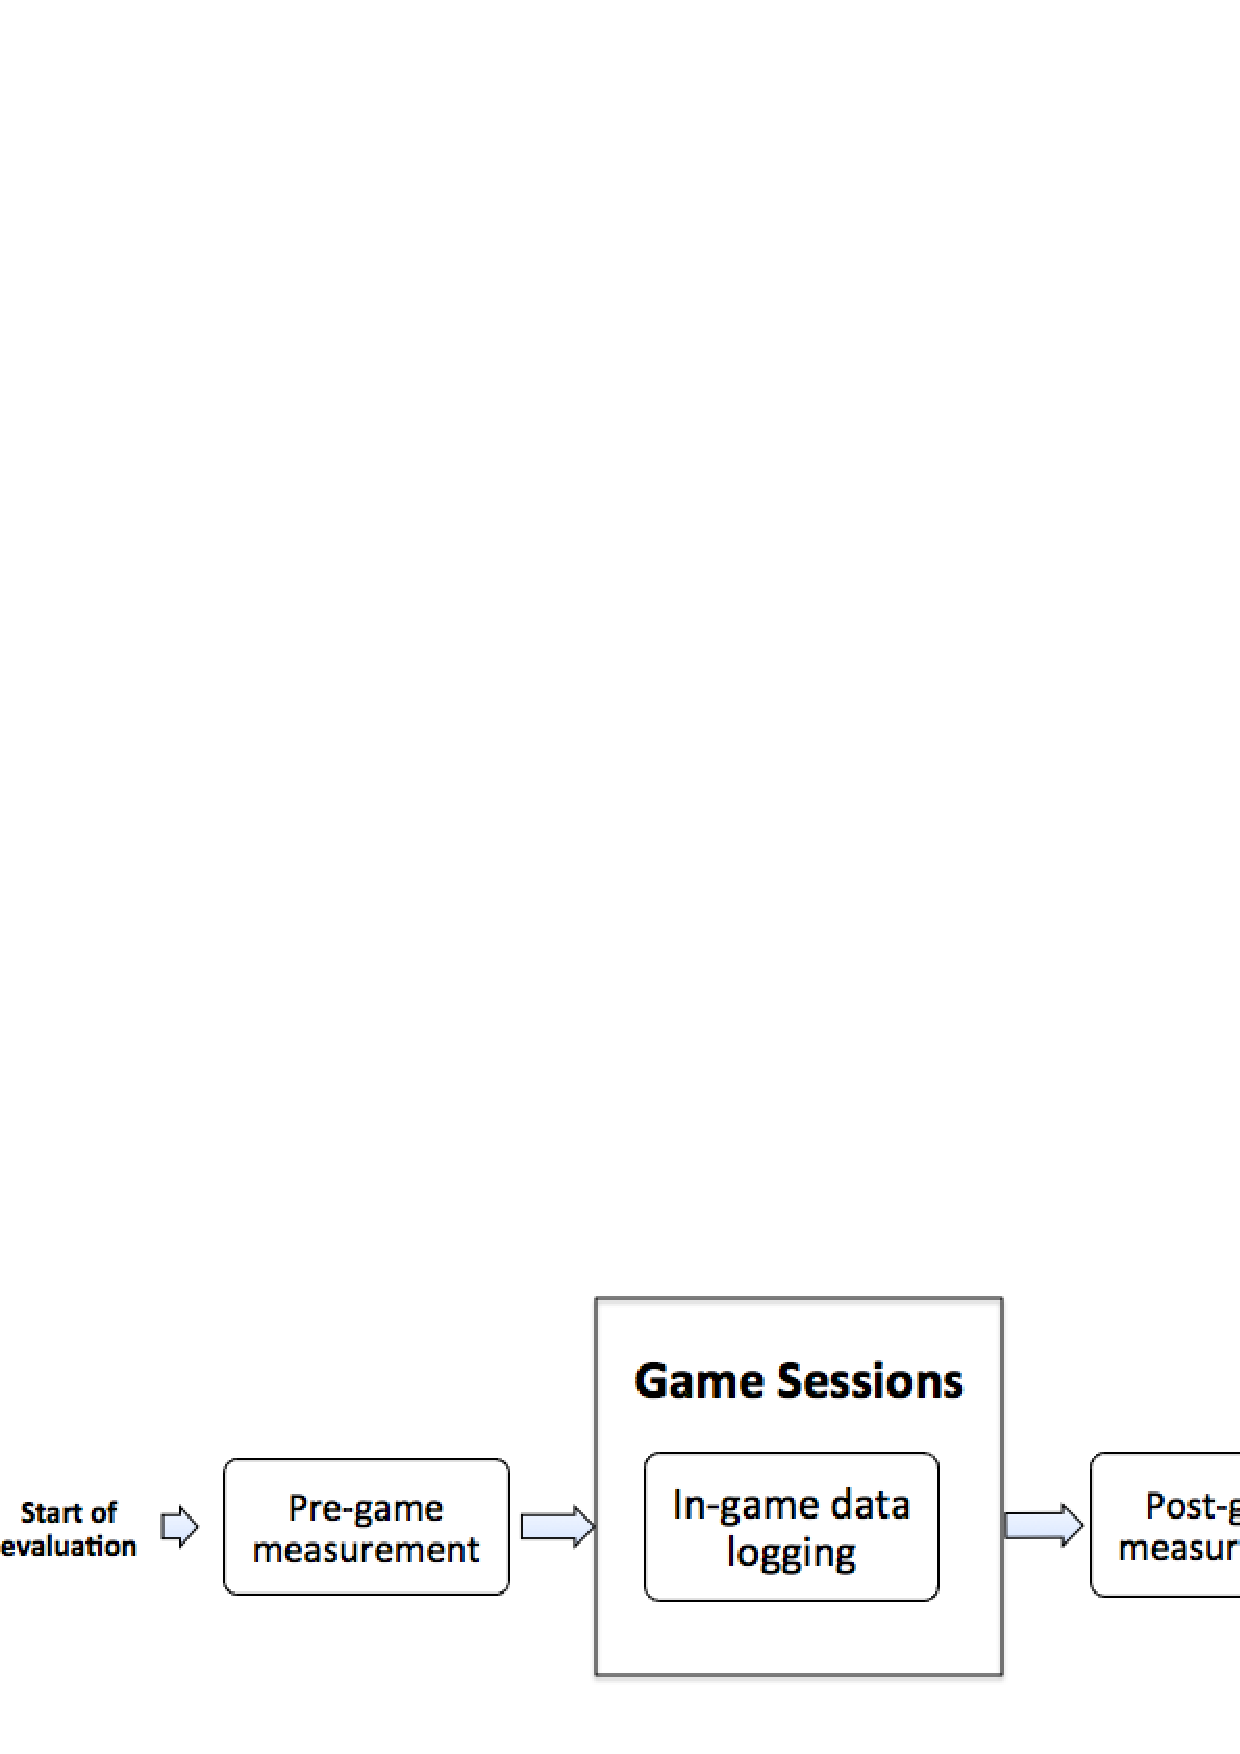
\includegraphics[width=3in]{pre-post-eval}
  \caption{Player Effectiveness Evaluation Process}
  \label{fig:pre-post-eval}
\end{figure}

\emph {(a) Literacy assessment:} One important goal of the serious
game for sustainability is the education effect on the
players. Literacy assessment is an indicator of such effect if there
is any.

SEE uses the similar approach described in \cite{csdl2-10-08} to
assess the player's sustainability literacy. A set of literacy survey
questionnaires (pre-game) will be presented to the players at the
beginning of or before the game. After the game ends, the same survey
(post-game) will then be presented to the players who responded the
pre-game survey. These two set of survey response data will be
compared to understand if there is any changes.

The extent of player's sustainability literacy change will indicate
the degree of educational effectiveness of the serious game for
sustainability.

\emph {(b) Behavior change assessment:} Positive behavior change is
another main goal of a serious game for sustainability. A serious game
for sustainability normally include some degree of resource
consumption measurement. SEE uses resource consumption data before and
after the game as part of the assessment for the result of the
player's sustainability behavior change.  The resource consumption
baseline prior to the game will be established based on historical
consumption data. During and after the game, we can compare the
resource consumption with the baseline for a particular day to
understand to what extent the resource consumption has changed.

The problems with using the baseline to assess the energy reduction in
the cases of dormitory energy challenge is discussed in details
here\cite{csdl2-12-08}.  As a framework for evaluating the
effectiveness of serious game for sustainability in a broader context
beyond the dormitory challenge, we continue to use the baseline
method as one way to assess the resource consumption reduction.

Besides using resource consumption change as one of the indicators of
the player's behavior change, we will give a behavior survey to the
players, to understand the change (if there is any). A pre-game survey
will be presented to the players to ask about their current
sustainability behavior, then after the game, a post-game survey to
ask about the player's behavior again. These two set of survey
response data will be compared to understand if there is any changes.

The combination of resource consumption changes and self-reported
behavior changes, will be used to understand the degree of behavior
effectiveness of the serious game for sustainability.

\emph {(c) Engagement assessment:} Player's engagement is an important
assessment to understand the effectiveness of a serious game. By
investigating the degree of engagement, we understand that the players
are actively participating in the game thus any changes in the
player's literacy and and behavior, are related to the participation
in the game, although we can not theoretically prove that the
participation cause the changes. On the other hand, if there is no or
little participation, we could safely deduce that if there is any
changes in sustainability literacy and behavior, they are mostly
caused by something else, not the serious game in question.

A serious game should include detailed log data for the players'
interaction with the game. The following are the player engagement
metrics we will measure:

\begin{itemize}
\item active participation rate
\item number of players per day
\item average session time
\item submissions per day
\item level of social engagement
\item website errors
\end{itemize}

\subsubsection{2. Game Designer Efficiency}

\emph{How efficient is it to design a game using the serious game
  framework?}

We will look at how much time it takes to design the game, and how
many errors the designers encountered during the design process.  The
serious game framework normally provides certain tools or interfaces
for the designers to design the game. This may involve configuring
global settings for the game, such as how long will the game run, who
are the players, and how to design individual game elements.

SEE proposes to first identify the list of design tasks, then look at
two set of data to assess the game designer's efficiency. One set of
data is the admin log data for the interaction between the game
designer and the serious game framework. From these log data, we could
derive the time it took a designer to complete a certain design task
using the game framework, and any system error he encountered. Another
set of data will be obtained by interviewing the designers to answer:
\begin{itemize}
    \item How much time did you spend to complete each design task?
    \item What problem did you encountered?
    \item Did you find it difficult to configure? what is difficult?
    \item Did you find it difficult to design a specific game? which
      one, what is difficult?
    \item What did you like the least when using the system?
\end{itemize}

\subsubsection{3. Game Manager Efficiency}

\emph{How efficient is it to manage the game using the serious game
  framework?}

To investigate how efficient it is to manage a game, we will look at
how much time it takes to manage the game, and how many errors the
game managers encountered during the process.  The serious game
frameworks normally provide certain interfaces for the managers to
manage the game. This may involve managing player submissions,
monitoring the game state, entering manual resource data, notifying
winners of the game, etc.

SEE proposes to first identify the list of managing tasks, then
analyze two sets of data to assess the game manager's efficiency. The
first set of data is the admin log data for the interaction between
the game manager and the serious game framework. From these log data,
we could derive the time it took a manager to complete a certain
managing task using the interface, and any system error he
encountered. The second set of data will be obtained by interviewing
the managers to answer:
\begin{itemize}
\item How much time did you spend to complete each managing task?
\item What problem did you encountered?
\item Did you find it difficult to manage? what is difficult?
\item What did you like the least when using the system?
\end{itemize}

It is possible that the same people share the role of game manager and
game designer, for example, the game designer also manages the
game. In this case, the evaluation will look at the same person's
data, both admin log and interview, with different assessing
questions.

\subsubsection{4. System Admin Efficiency}

\emph{How efficient is it to install and maintain the system?}

To investigate how efficient it is to install and maintain
the game, we will look at how much time it takes to install and
maintain the game, and how many errors encountered during the
process. To investigate these two areas we will interview the system
admin to answer:
\begin{itemize}
\item How much time did you spend to install the system?
\item How much time did you spend to maintain the system?
\item What problem did you encountered?
\item Did you find it difficult to admin the system? what is difficult?
\item What did you like the least about administrating the system?
\end{itemize}

\subsubsection{5. Developer Efficiency}

\emph{How efficient is it to understand, extend and debug the system?}

To investigate how efficient it is to understand, extend and debug the
system, we will look at how much time it takes to develop an
enhancement to the game framework, and how many errors encountered
during the process. We will interview the developer(s) to
answer:
\begin{itemize}
\item How much time did you spend to set up the development
  environment?
\item How much time did you spend developing and debugging an
  enhancement to the game framework?
\item What problem(s) did you encounter?
\item Did you find it difficult to understand, extend and debug the
  system? What was difficult?
\item What did you like the least when developing the game
  enhancement? 
\end{itemize}

\subsubsection{6. Researcher Efficiency}

\emph{How efficient is it to do research with the system?}

To investigate how efficient it is to do research with the system, we
will look at how much time it takes to use the system for specific
research query, and how many errors encountered during the process. We
will interview the researcher(s) to answer:
\begin{itemize}
\item How much time did you spend to collect the research data for a
  specific topic?
\item What problem did you encountered when collecting the data?
\item Did you find the data you collect helpful to your research? if
  not, what can be improved?
\item Did you find it difficult to collect the data from the system?
  what is difficult?
\item What did you like the least about using the system?
\end{itemize}

\section{Case Study of Makahiki}

Now that we had described the SEE framework, this section will discuss
the case study of how we applied SEE to evaluate the Makahiki serious
game framework for sustainability. First we will first describe the
Makahiki framework.

\subsection{Makahiki in Brief}

We developed an innovative serious game framework for sustainability
called Makahiki. It is an IT infrastructure for the development of
sustainability challenges. Makahiki explores one section of the design
space where virtual world game mechanics are employed to affect real
world sustainability behaviors.

Makahiki consists of a configurable game engine that can be customized
to the needs of different organizations.  It includes a library of
pre-built game ``widgets'' that implement a variety of game mechanics.
Using the widgets, an organization can create a custom energy % CAM:
                                % we suddenly switch from
                                % sustainability to energy.
challenge in which players can compete individually and/or in teams to
earn the most points by reducing their energy consumption as well as
by learning about energy concepts in general. Figure
\ref{fig:makahiki-architecture} illustrates the architecture of
Makahiki. Figure \ref{fig:makahiki-games} shows a few examples of the
games implemented in the Makahiki game library. More detailed
description of Makahiki can be found here \cite{csdl2-12-06}.

\begin{figure}
  \center
  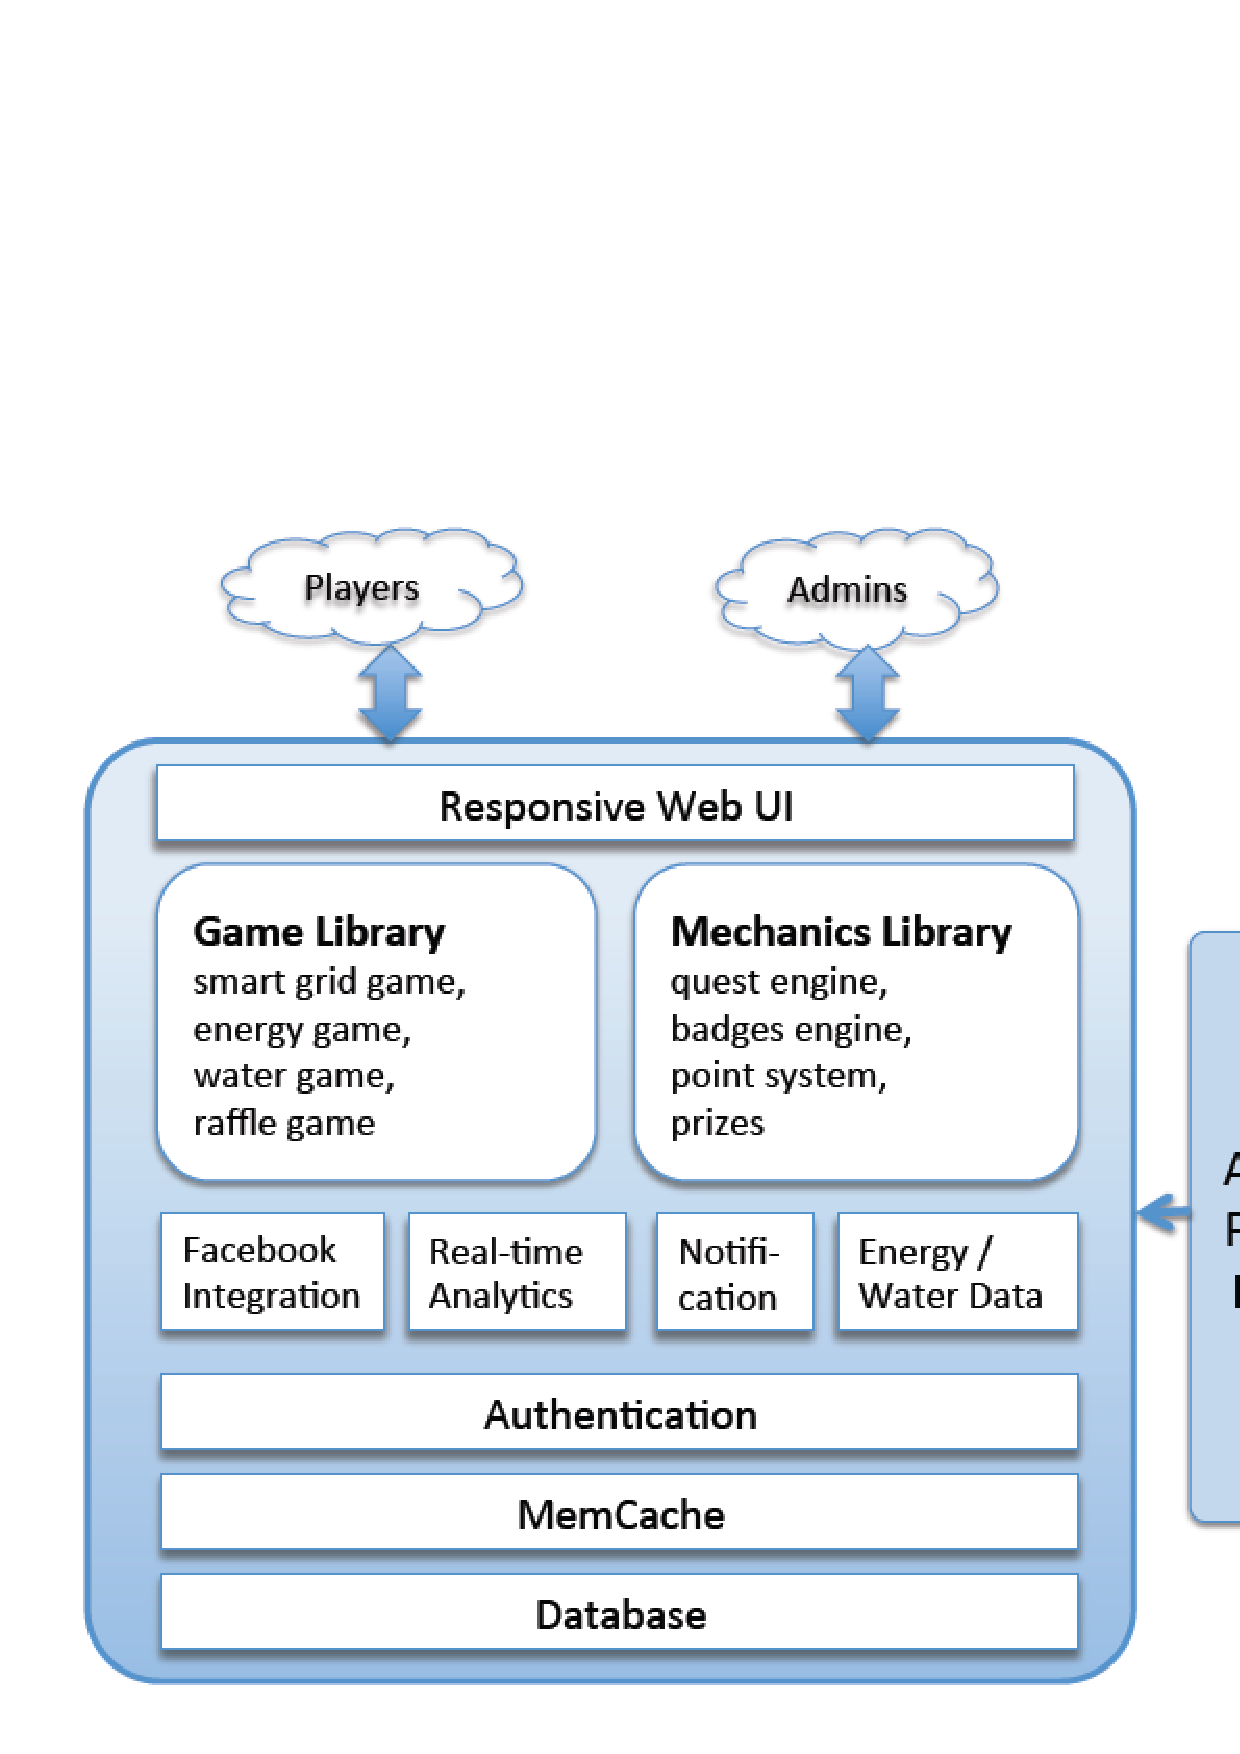
\includegraphics[width=3in]{makahiki-system-architecture}
  \caption{Architecture of Makahiki}
  \label{fig:makahiki-architecture}
\end{figure}

\begin{figure}
	\center
		\subfigure[Smart Grid Game]{\label{fig:SmartGrid}\includegraphics[width=1.5in,height=1.2in]{smart-grid-game.eps}}
		\subfigure[Energy Goal Game]{\label{fig:DailyEnergyGoal}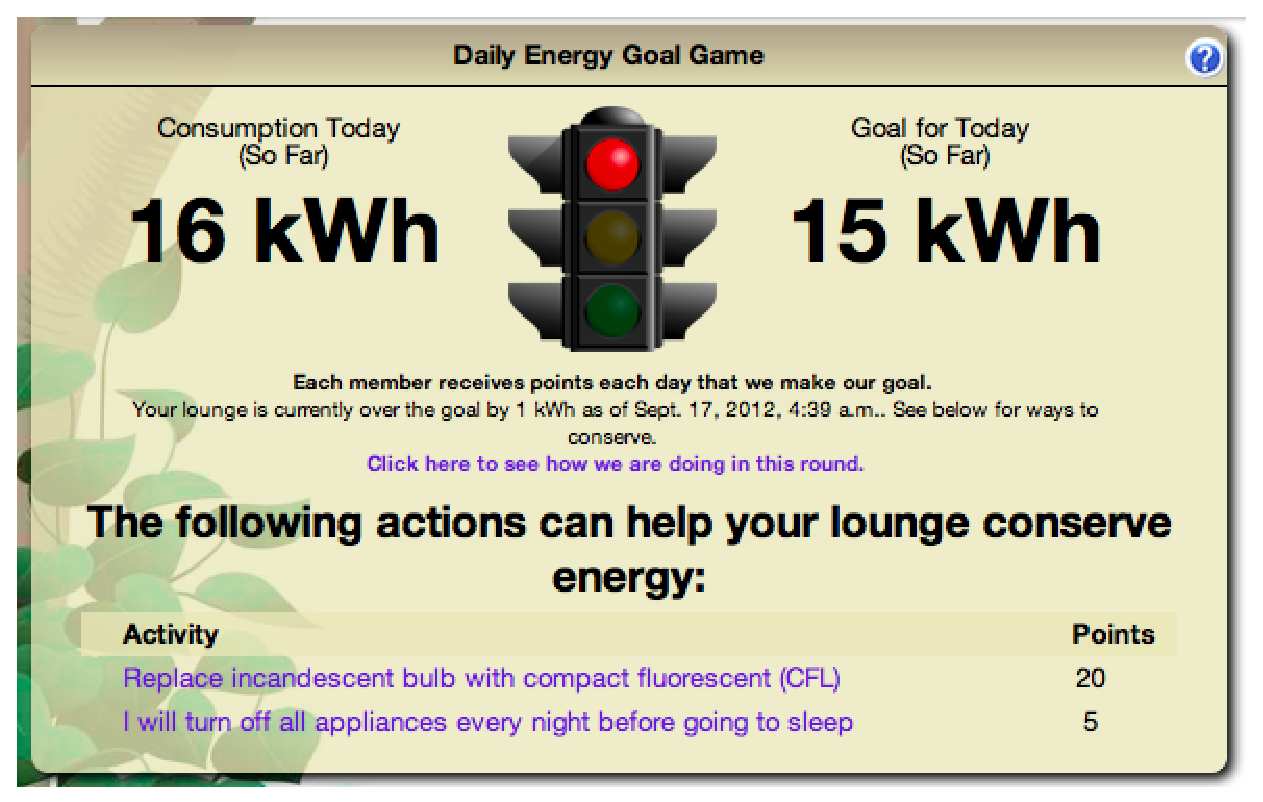
\includegraphics[width=1.5in,height=1.2in]{daily-energy-goal-game.eps}}
		\caption{Makahiki Game Library}
		\label{fig:makahiki-games}
\end{figure}

\subsection{Experiences with Makahiki}

We have used Makahiki in the real world to create four different Kukui
Cup Energy Challenges. The first and second Kukui Cup Energy challenge
of University of Hawaii was held in 2011 and 2012 for over 1,000 first
year students living in the residence halls. Hawaii Pacific University
(HPU) held a Kukui Cup Energy challenge in Fall 2012 for about 200
students. An international organization called the East-West Center
(EWC) held a Kukui Cup Energy and Water challenge for the
international residents living in the resident halls without smart
meters, so the resource consumption data had to be entered by the game
mangers manually.

The successful creation of serious game challenges by three different
organizations provides evidence that the Makahiki serious game engine
can be tailored to the differing needs of separate
organizations. First, UH uses smart meters by Electro-Industries Inc.,
while HPU uses smart meters by EGauge Inc., and EWC collected their
energy data manually. Second, while UH and HPU challenges involved
only energy consumption data, the EWC challenge involved both energy
and water consumption data (which was also collected manually).
Third, the IT infrastructure at UH and HPU provided authentication
services using CAS and LDAP, while EWC used the built-in Django
authentication. Fourth, the user interface was customized to ``brand''
each challenge with the logo, thematic elements, and the education
contents of the sponsoring organizations.

Besides the real world usage of Makahiki in the series Kukui Cup
challenge, We also performed in-lab evaluation experiments. Makahiki
was used in the serious game development course at the University of
Hawaii. The students were seniors or graduate students majored in the
computer science related fields. During the course, the students 
installed Makahiki, configured and designed a serious game instance with
Makahiki, and finally developed an enhancement to the Makahiki
framework. We asked the students taking the course to voluntarily
participate in the evaluation experiments of Makahiki, using SEE.

\subsection{Evaluation of Makahiki}

This section describes the details of Makahiki evaluation using SEE.

\subsubsection{Player Effectiveness}

We evaluated player effectiveness using the 2012 Kukui Cup instance at
the University of Hawaii at Manoa. There were over 1000 eligible
players for this instances. They were the first year college student
living in four similar structured resident halls in close
vicinity. Makahiki recorded detailed logging data from every
interaction between the players and the website. 

\emph{To what extend does the game increase player's literacy in
  sustainability?}

We conducted the two surveys, one before the challenge (pre-game) and
one after the challenge (post-game). The players' sustainability
literacy and behavior change was:
% CAM: need to put in some preliminary results.

\emph{To what extent does the game produce positive player behavior
  change in sustainability?}

The energy consumption data before, during and after the challenge were
examined to understand any usage pattern or reduction during and after
the challenge. The results were:
% CAM: need to put in some preliminary results.

\emph{To what extent does the game engage players?}

We calculated the engagement metrics and the results were:
% CAM: need to put in some preliminary results.


\subsubsection{Game Manager Efficiency Evaluation}

Game manager efficiency evaluation was performed by interviewing the
game managers of the Hawaii Pacific University and East-West Center at
Hawaii challenges. The interviews took place after the challenge. We
asked them about their experiences in using the Makahiki admin
interface for the managing process during the challenge. The admin
interface log data is also analyzed to assess if there is any error
encountered during the challenge management.
% CAM: need to put in some preliminary results.


\subsubsection{System Admin Efficiency Evaluation}

System admin efficiency evaluation was performed in an in-lab
experiment. Students were tasked with installing the Makahiki
system into their local computers as well as the cloud environment. In
order to understand how much time it takes to install the Makahiki and
what problems might be encountered, We designed a Google form which
details the steps of installing Makahiki both locally and in the
cloud, and for each step, we asked the students to record the time
they spent and the problems they encountered.

Figure \ref{fig:makahiki-eval-form} illustrates a partial google form
used for Makahiki system admin evaluation.

\begin{figure}[ht!]
   \centering
   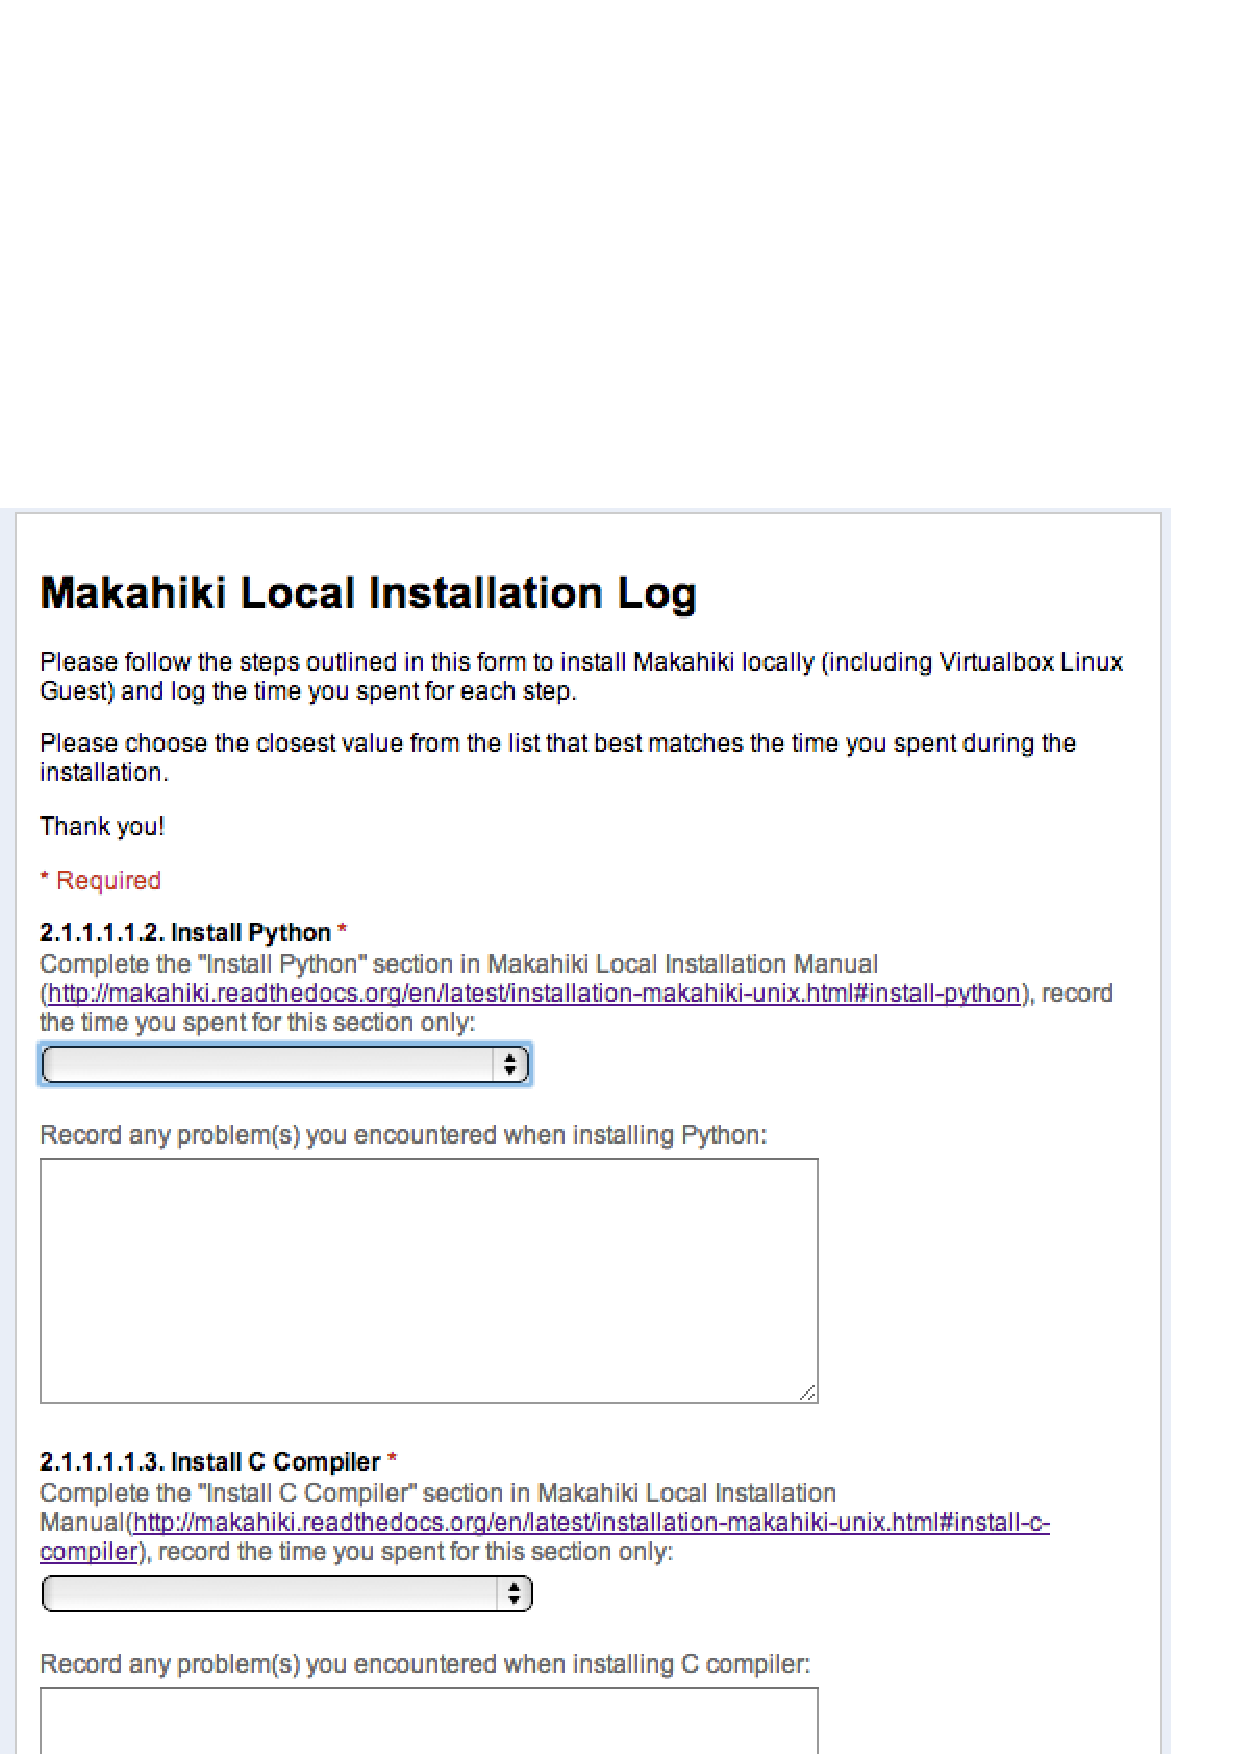
\includegraphics[width=3.5in]{developer-eval-form}
   \caption{Makahiki Evaluation Form}
   \label{fig:makahiki-eval-form}
\end{figure}

We also asked the students to provide feedback about their
installation experiences in the form of blog post.
% CAM: need to put in some preliminary results.

\subsubsection{Game Designer Efficiency Evaluation}

Another class assignment for students was to design a Kukui Cup like
serious game using Makahiki. We asked the students to follow specific
design steps and record their time and problem encountered during
their design process.

Students were also asked to provide feedback about their design
experiences in the form of blog post.

Game designer efficiency evaluation was also performed by interviewing
the game designers of the Hawaii Pacific University and East-West
Center at Hawaii challenges. The interviews took place before the
challenge starts to capture their experiences in using the Makahiki
admin interface for the design process, which normally happen before
the challenge. We analyzed both the qualitative data collected from
the interviews and email changes with the game managers, and the
quantitative collected from the admin interface log data.
% CAM: need to put in some preliminary results.

\subsubsection{Developer Efficiency Evaluation}

The students were tasked with developing an enhancement to the
Makahiki instance. This involved setting up the development
environment, following the tutorial to create the "Hello world" widget
using Makahiki, and finally, developing an enhancement which extended
the functionality of Makahiki.

The students were asked to submit their development source code to the
public source code repository (Github) and write a blog post to
discuss their efforts to complete the development activity.

We reviewed their source code to compare their code to the reference
implementation, analyzed the blog post from the students, as well as
any email correspondence from students discussing the problem in the
development.
% CAM: need to put in some preliminary results.

\subsubsection{Researcher Experience Evaluation}

We interviewed the researchers using the University of Hawaii
instance.
% CAM: need to put in some preliminary results.

\section{Conclusion}

We developed a serious game framework evaluation mechanism called
Stakeholder Experience Evaluation (SEE). SEE evaluates serious game
frameworks from the perspective of different stakeholders'
experiences; player effectiveness, game designers efficiency, game
managers efficiency, system administrators efficiency, developers
efficiency, and researchers efficiency. These experiences are
evaluated qualitatively and quantitatively to evaluate the serious
game framework.

We also applied the SEE evaluation mechanism to Makahiki. The results
show that ...

\section{Future Work}

The development of SEE framework creates another research question:
what are the strengths and weaknesses of this evaluation framework? To
answer that question, we are planing to apply the evaluation framework
to another serious game framework (such as the
commercial Lucid Dashboard system \cite{building-dashboard}). With the
insights gained from another case study, SEE can be further
improved.

One area of effectiveness evaluation is currently not addressed in the
SEE framework: the longitudinal evaluation of player effectiveness.
We want to find out whether the serious game experience actually had
lasting impacts on players. In the context of Makahiki-based serious
games for sustainability, whether the student players were able to
continue any positive sustainability behaviors after leaving their
residence halls.

\section{Acknowledgments}
Omitted from review version.

%\textbf{Don't forget
%to acknowledge funding sources as well}, so you don't wind up
%having to correct it later.

% Balancing columns in a ref list is a bit of a pain because you
% either use a hack like flushend or balance, or manually insert
% a column break.  http://www.tex.ac.uk/cgi-bin/texfaq2html?label=balance
% multicols doesn't work because we're already in two-column mode,
% and flushend isn't awesome, so I choose balance.  See this
% for more info: http://cs.brown.edu/system/software/latex/doc/balance.pdf
%
% Note that in a perfect world balance wants to be in the first
% column of the last page.
%
% If balance doesn't work for you, you can remove that and
% hard-code a column break into the bbl file right before you
% submit:
%
% http://stackoverflow.com/questions/2149854/how-to-manually-equalize-columns-
% in-an-ieee-paper-if-using-bibtex
%
% Or, just remove \balance and give up on balancing the last page.
%
\balance

% If you want to use smaller typesetting for the reference list,
% uncomment the following line:
% \small
\bibliographystyle{acm-sigchi}
\bibliography{sustainability,csdl-trs,gamification,13-03}
\end{document}
